\chapter{Overview}
\label{sec:design_overview}
This section presents an overview of the design work done on the overall product, and the following sections present details on specific features in the launcher. \newline

The design of the \giraf[] launcher is centered around high usability and specific functionality requirements. 
These functionality requirements come from both the customers of the project, and other \localgroup[]s in the multi project, and include only the requirements that are within the scope of this project. \newline
The requirements are as follows:
\begin{itemize}
\item Allow \guardian[]s to launch apps.
\item Allow each \guardian[] to customize their experience with the launcher. 
\item Allow apps to work for a specific \autist[].
\end{itemize}

High usability has been prioritized, both because it was requested by the customer, but also because the launcher is planned to be expanded and usable by \autists[] later on.
See \autoref{Preanalysis:Usability_for_children} for more information on the usability requirements of children. \newline

The above requirements have resulted in an overall interaction design, which can be seen in \autoref{fig:state_diagram}, in the form of a state diagram.

\begin{figure}[h]
	\centering
	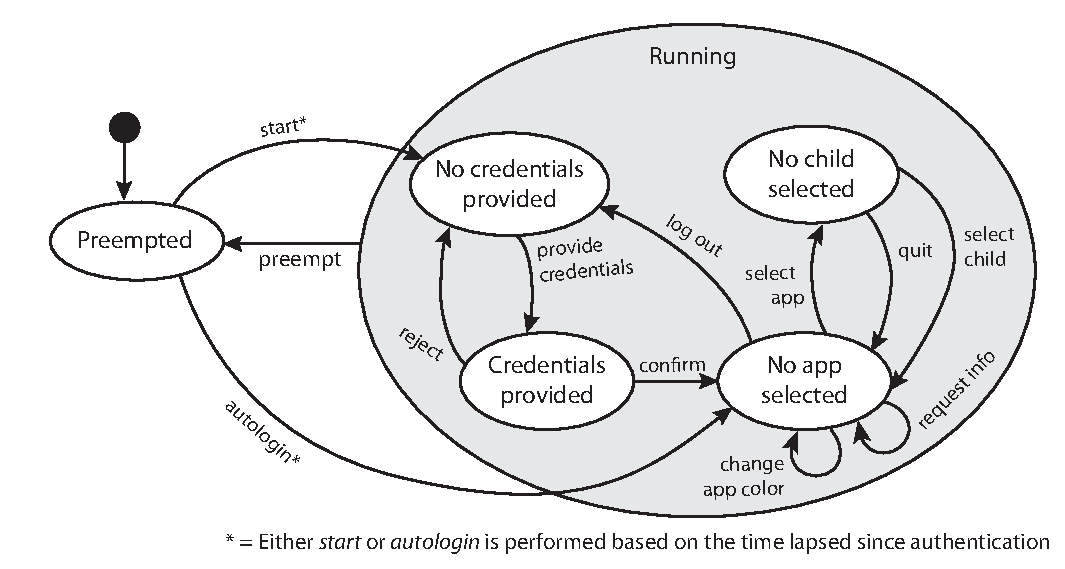
\includegraphics[width=1\textwidth]{gfx/statediagram.pdf}
	\caption{State diagram showing the states and actions of the system.}
	\label{fig:state_diagram}
\end{figure}

To make the design easier to approach, the system is split into four distinct features: Authentication, app management, profile selection, and resumption. 
This split is illustrated in \autoref{fig:design_diagram}, which groups the states and actions of \autoref{fig:state_diagram} according to their to the feature they belong to. 

\begin{figure}[h]
	\centering
	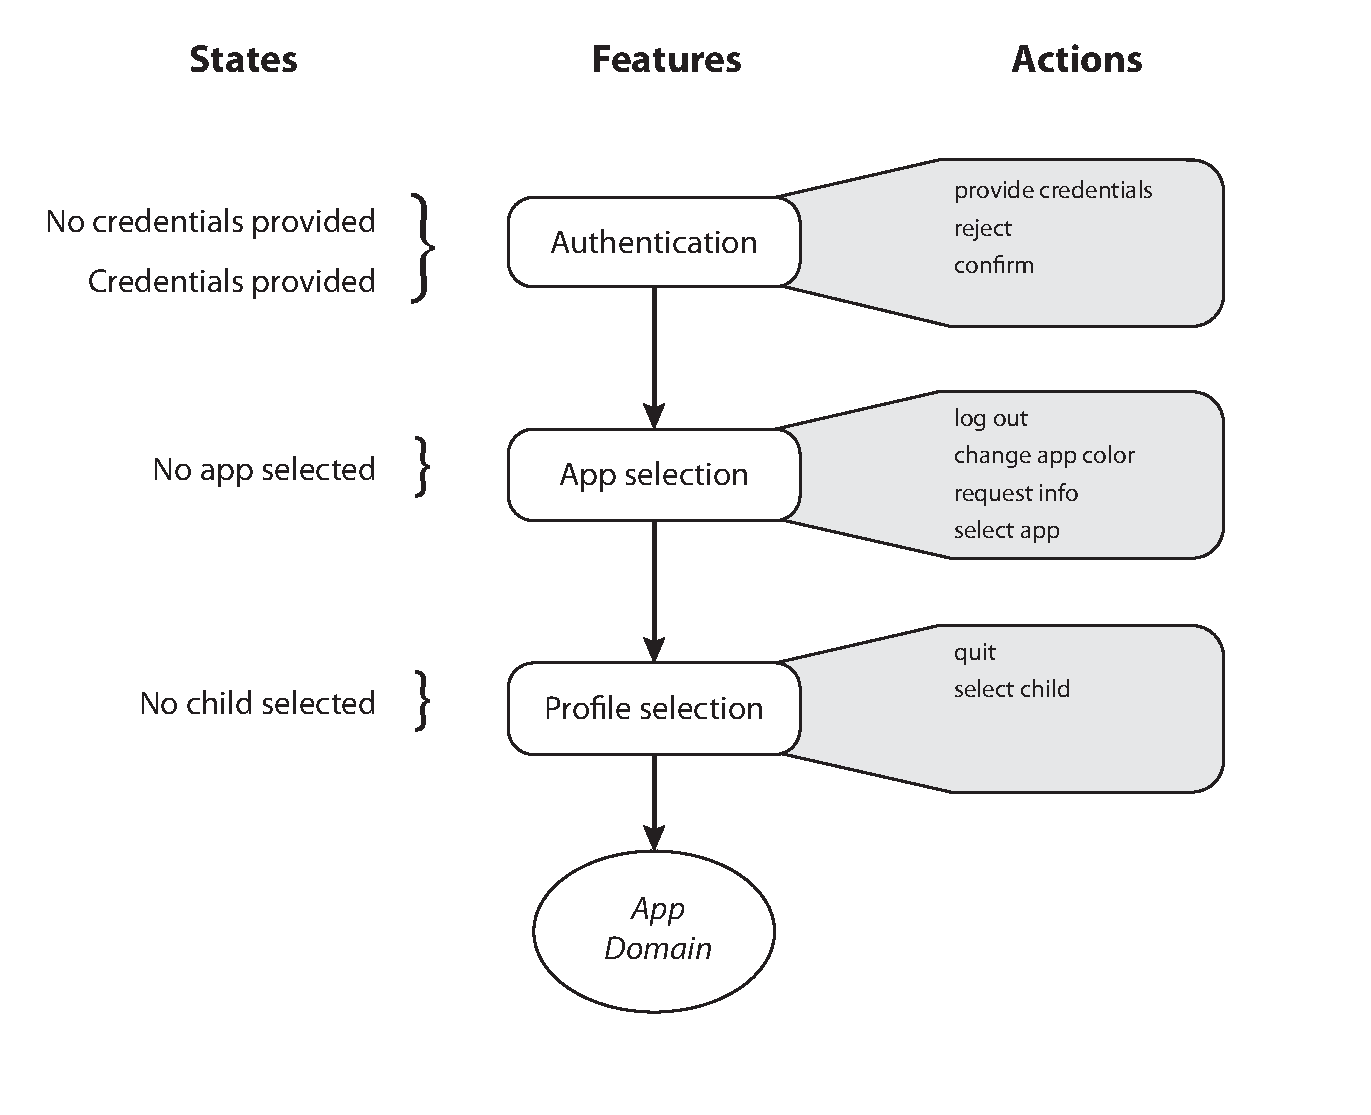
\includegraphics[width=1\textwidth]{gfx/design_diagram.pdf}
	\caption{Design diagram illustrating the three features of the system.}
	\label{fig:design_diagram}
\end{figure}